% Options for packages loaded elsewhere
\PassOptionsToPackage{unicode}{hyperref}
\PassOptionsToPackage{hyphens}{url}
%
\documentclass[
  12pt,
]{article}
\title{Precipitation Change in Beaufort, NC}
\usepackage{etoolbox}
\makeatletter
\providecommand{\subtitle}[1]{% add subtitle to \maketitle
  \apptocmd{\@title}{\par {\large #1 \par}}{}{}
}
\makeatother
\subtitle{\url{https://github.com/tarokatayama/KatayamaNgenziThornton_ENV872_EDA_FinalProject.git}}
\author{Karen Thornton, Lambert Ngenzi, Taro Katayama}
\date{}

\usepackage{amsmath,amssymb}
\usepackage{lmodern}
\usepackage{iftex}
\ifPDFTeX
  \usepackage[T1]{fontenc}
  \usepackage[utf8]{inputenc}
  \usepackage{textcomp} % provide euro and other symbols
\else % if luatex or xetex
  \usepackage{unicode-math}
  \defaultfontfeatures{Scale=MatchLowercase}
  \defaultfontfeatures[\rmfamily]{Ligatures=TeX,Scale=1}
  \setmainfont[]{Times New Roman}
\fi
% Use upquote if available, for straight quotes in verbatim environments
\IfFileExists{upquote.sty}{\usepackage{upquote}}{}
\IfFileExists{microtype.sty}{% use microtype if available
  \usepackage[]{microtype}
  \UseMicrotypeSet[protrusion]{basicmath} % disable protrusion for tt fonts
}{}
\makeatletter
\@ifundefined{KOMAClassName}{% if non-KOMA class
  \IfFileExists{parskip.sty}{%
    \usepackage{parskip}
  }{% else
    \setlength{\parindent}{0pt}
    \setlength{\parskip}{6pt plus 2pt minus 1pt}}
}{% if KOMA class
  \KOMAoptions{parskip=half}}
\makeatother
\usepackage{xcolor}
\IfFileExists{xurl.sty}{\usepackage{xurl}}{} % add URL line breaks if available
\IfFileExists{bookmark.sty}{\usepackage{bookmark}}{\usepackage{hyperref}}
\hypersetup{
  pdftitle={Precipitation Change in Beaufort, NC},
  pdfauthor={Karen Thornton, Lambert Ngenzi, Taro Katayama},
  hidelinks,
  pdfcreator={LaTeX via pandoc}}
\urlstyle{same} % disable monospaced font for URLs
\usepackage[margin=2.54cm]{geometry}
\usepackage{color}
\usepackage{fancyvrb}
\newcommand{\VerbBar}{|}
\newcommand{\VERB}{\Verb[commandchars=\\\{\}]}
\DefineVerbatimEnvironment{Highlighting}{Verbatim}{commandchars=\\\{\}}
% Add ',fontsize=\small' for more characters per line
\usepackage{framed}
\definecolor{shadecolor}{RGB}{248,248,248}
\newenvironment{Shaded}{\begin{snugshade}}{\end{snugshade}}
\newcommand{\AlertTok}[1]{\textcolor[rgb]{0.94,0.16,0.16}{#1}}
\newcommand{\AnnotationTok}[1]{\textcolor[rgb]{0.56,0.35,0.01}{\textbf{\textit{#1}}}}
\newcommand{\AttributeTok}[1]{\textcolor[rgb]{0.77,0.63,0.00}{#1}}
\newcommand{\BaseNTok}[1]{\textcolor[rgb]{0.00,0.00,0.81}{#1}}
\newcommand{\BuiltInTok}[1]{#1}
\newcommand{\CharTok}[1]{\textcolor[rgb]{0.31,0.60,0.02}{#1}}
\newcommand{\CommentTok}[1]{\textcolor[rgb]{0.56,0.35,0.01}{\textit{#1}}}
\newcommand{\CommentVarTok}[1]{\textcolor[rgb]{0.56,0.35,0.01}{\textbf{\textit{#1}}}}
\newcommand{\ConstantTok}[1]{\textcolor[rgb]{0.00,0.00,0.00}{#1}}
\newcommand{\ControlFlowTok}[1]{\textcolor[rgb]{0.13,0.29,0.53}{\textbf{#1}}}
\newcommand{\DataTypeTok}[1]{\textcolor[rgb]{0.13,0.29,0.53}{#1}}
\newcommand{\DecValTok}[1]{\textcolor[rgb]{0.00,0.00,0.81}{#1}}
\newcommand{\DocumentationTok}[1]{\textcolor[rgb]{0.56,0.35,0.01}{\textbf{\textit{#1}}}}
\newcommand{\ErrorTok}[1]{\textcolor[rgb]{0.64,0.00,0.00}{\textbf{#1}}}
\newcommand{\ExtensionTok}[1]{#1}
\newcommand{\FloatTok}[1]{\textcolor[rgb]{0.00,0.00,0.81}{#1}}
\newcommand{\FunctionTok}[1]{\textcolor[rgb]{0.00,0.00,0.00}{#1}}
\newcommand{\ImportTok}[1]{#1}
\newcommand{\InformationTok}[1]{\textcolor[rgb]{0.56,0.35,0.01}{\textbf{\textit{#1}}}}
\newcommand{\KeywordTok}[1]{\textcolor[rgb]{0.13,0.29,0.53}{\textbf{#1}}}
\newcommand{\NormalTok}[1]{#1}
\newcommand{\OperatorTok}[1]{\textcolor[rgb]{0.81,0.36,0.00}{\textbf{#1}}}
\newcommand{\OtherTok}[1]{\textcolor[rgb]{0.56,0.35,0.01}{#1}}
\newcommand{\PreprocessorTok}[1]{\textcolor[rgb]{0.56,0.35,0.01}{\textit{#1}}}
\newcommand{\RegionMarkerTok}[1]{#1}
\newcommand{\SpecialCharTok}[1]{\textcolor[rgb]{0.00,0.00,0.00}{#1}}
\newcommand{\SpecialStringTok}[1]{\textcolor[rgb]{0.31,0.60,0.02}{#1}}
\newcommand{\StringTok}[1]{\textcolor[rgb]{0.31,0.60,0.02}{#1}}
\newcommand{\VariableTok}[1]{\textcolor[rgb]{0.00,0.00,0.00}{#1}}
\newcommand{\VerbatimStringTok}[1]{\textcolor[rgb]{0.31,0.60,0.02}{#1}}
\newcommand{\WarningTok}[1]{\textcolor[rgb]{0.56,0.35,0.01}{\textbf{\textit{#1}}}}
\usepackage{longtable,booktabs,array}
\usepackage{calc} % for calculating minipage widths
% Correct order of tables after \paragraph or \subparagraph
\usepackage{etoolbox}
\makeatletter
\patchcmd\longtable{\par}{\if@noskipsec\mbox{}\fi\par}{}{}
\makeatother
% Allow footnotes in longtable head/foot
\IfFileExists{footnotehyper.sty}{\usepackage{footnotehyper}}{\usepackage{footnote}}
\makesavenoteenv{longtable}
\usepackage{graphicx}
\makeatletter
\def\maxwidth{\ifdim\Gin@nat@width>\linewidth\linewidth\else\Gin@nat@width\fi}
\def\maxheight{\ifdim\Gin@nat@height>\textheight\textheight\else\Gin@nat@height\fi}
\makeatother
% Scale images if necessary, so that they will not overflow the page
% margins by default, and it is still possible to overwrite the defaults
% using explicit options in \includegraphics[width, height, ...]{}
\setkeys{Gin}{width=\maxwidth,height=\maxheight,keepaspectratio}
% Set default figure placement to htbp
\makeatletter
\def\fps@figure{htbp}
\makeatother
\setlength{\emergencystretch}{3em} % prevent overfull lines
\providecommand{\tightlist}{%
  \setlength{\itemsep}{0pt}\setlength{\parskip}{0pt}}
\setcounter{secnumdepth}{5}
\ifLuaTeX
  \usepackage{selnolig}  % disable illegal ligatures
\fi

\begin{document}
\maketitle

\newpage
\tableofcontents
\newpage
\DataWrangling
\newpage
\listoffigures 
\newpage

\hypertarget{rationale-and-research-questions}{%
\section{Rationale and Research
Questions}\label{rationale-and-research-questions}}

Question 1: Has there been a significant increase in precipitation in
Beaufort, NC from 1980 to 2016?

Question 2: Has there been a significant increase in 1-year/24h
precipitation event in Beaufort, NC from decade to decade (1997 to 2006
and 2007 to 2016)?

Null Hypothesis 1: There is no significant change in precipitation from
1980 to 2016.

Null Hypothesis 2: There is no significant change in 1-year/24h
precipitation events from decade to decade (1997 to 2006 and 2007 to
2016).

\newpage

\hypertarget{dataset-information}{%
\section{Dataset Information}\label{dataset-information}}

Data was originally attained online from DAYMET for a Hydrology
assignment during Fall Semester. Since then, DAYMET has been taken down,
so the excel sheet from class was used. The data shows historical
precipitation data from Beaufort, NC for the years 1980 to 2016.

``Significant 1-year/24hr Precipitation Events'' are considered 1
year/24h events using the NOAA threshold of 3.66 inches. This means that
in 24h the probability of it raining 3.66 inches should only happen once
a year. These events are considered large storm events.

\begin{Shaded}
\begin{Highlighting}[]
\CommentTok{\# Load your datasets}
\NormalTok{Beaufort\_RAW}\OtherTok{\textless{}{-}}\FunctionTok{read.csv}\NormalTok{(}\StringTok{"./Data/Beaufort\_precip\_1980{-}present\_HUC\_030203010503\_dayMet\_split{-}dates{-}columns.csv"}\NormalTok{, }\AttributeTok{stringsAsFactors =} \ConstantTok{TRUE}\NormalTok{)}
\end{Highlighting}
\end{Shaded}

\newpage

\hypertarget{exploratory-analysis}{%
\section{Exploratory Analysis}\label{exploratory-analysis}}

Load all packages and get the working directory

\begin{Shaded}
\begin{Highlighting}[]
\CommentTok{\# Set your working directory}
\FunctionTok{getwd}\NormalTok{()}
\end{Highlighting}
\end{Shaded}

\begin{verbatim}
## [1] "/Users/tarokatayama/Desktop/Duke_Semester_2/Environmental_data_analytics/R_Projects/KatayamaNgenziThornton_ENV872_EDA_FinalProject"
\end{verbatim}

\begin{Shaded}
\begin{Highlighting}[]
\CommentTok{\# Load your packages}
\FunctionTok{library}\NormalTok{(webshot)}
\FunctionTok{library}\NormalTok{(tidyverse)}
\end{Highlighting}
\end{Shaded}

\begin{verbatim}
## -- Attaching packages --------------------------------------- tidyverse 1.3.1 --
\end{verbatim}

\begin{verbatim}
## v ggplot2 3.3.5     v purrr   0.3.4
## v tibble  3.1.4     v dplyr   1.0.7
## v tidyr   1.1.3     v stringr 1.4.0
## v readr   2.0.1     v forcats 0.5.1
\end{verbatim}

\begin{verbatim}
## -- Conflicts ------------------------------------------ tidyverse_conflicts() --
## x dplyr::filter() masks stats::filter()
## x dplyr::lag()    masks stats::lag()
\end{verbatim}

\begin{Shaded}
\begin{Highlighting}[]
\FunctionTok{library}\NormalTok{(dplyr)}
\FunctionTok{library}\NormalTok{(lubridate)}
\end{Highlighting}
\end{Shaded}

\begin{verbatim}
## 
## Attaching package: 'lubridate'
\end{verbatim}

\begin{verbatim}
## The following objects are masked from 'package:base':
## 
##     date, intersect, setdiff, union
\end{verbatim}

\begin{Shaded}
\begin{Highlighting}[]
\FunctionTok{library}\NormalTok{(mapview)}
\FunctionTok{mapviewOptions}\NormalTok{(}\AttributeTok{fgb =} \ConstantTok{FALSE}\NormalTok{)}
\FunctionTok{library}\NormalTok{(sf)}
\end{Highlighting}
\end{Shaded}

\begin{verbatim}
## Warning: package 'sf' was built under R version 4.1.2
\end{verbatim}

\begin{verbatim}
## Linking to GEOS 3.9.1, GDAL 3.4.0, PROJ 8.1.1; sf_use_s2() is TRUE
\end{verbatim}

\begin{Shaded}
\begin{Highlighting}[]
\FunctionTok{library}\NormalTok{(knitr)}
\end{Highlighting}
\end{Shaded}

\begin{verbatim}
## Warning: package 'knitr' was built under R version 4.1.2
\end{verbatim}

\begin{Shaded}
\begin{Highlighting}[]
\FunctionTok{library}\NormalTok{(Kendall)}
\FunctionTok{library}\NormalTok{(zoo)}
\end{Highlighting}
\end{Shaded}

\begin{verbatim}
## 
## Attaching package: 'zoo'
\end{verbatim}

\begin{verbatim}
## The following objects are masked from 'package:base':
## 
##     as.Date, as.Date.numeric
\end{verbatim}

\begin{Shaded}
\begin{Highlighting}[]
\FunctionTok{library}\NormalTok{(gridExtra)}
\end{Highlighting}
\end{Shaded}

\begin{verbatim}
## 
## Attaching package: 'gridExtra'
\end{verbatim}

\begin{verbatim}
## The following object is masked from 'package:dplyr':
## 
##     combine
\end{verbatim}

\begin{Shaded}
\begin{Highlighting}[]
\FunctionTok{options}\NormalTok{(}\AttributeTok{scipen =} \DecValTok{4}\NormalTok{) }\CommentTok{\# limit number of digits }
\end{Highlighting}
\end{Shaded}

\hypertarget{initial-wrangling}{%
\section{Initial Wrangling}\label{initial-wrangling}}

\begin{Shaded}
\begin{Highlighting}[]
\CommentTok{\# Rename columns to logical names}
\FunctionTok{names}\NormalTok{(Beaufort\_RAW)[}\DecValTok{1}\NormalTok{] }\OtherTok{\textless{}{-}} \StringTok{"Date"}
\FunctionTok{names}\NormalTok{(Beaufort\_RAW)[}\DecValTok{2}\NormalTok{] }\OtherTok{\textless{}{-}} \StringTok{"Mean\_Precip\_mm"}

\CommentTok{\#Set Date as a Date}
\NormalTok{Beaufort\_RAW}\SpecialCharTok{$}\NormalTok{Date}\OtherTok{\textless{}{-}}\FunctionTok{as.Date}\NormalTok{(Beaufort\_RAW}\SpecialCharTok{$}\NormalTok{Date, }\StringTok{"\%Y{-}\%m{-}\%d"}\NormalTok{) }

\CommentTok{\# Set your ggplot theme}
\NormalTok{Theme }\OtherTok{\textless{}{-}} \FunctionTok{theme\_classic}\NormalTok{(}\AttributeTok{base\_size =} \DecValTok{7}\NormalTok{) }\SpecialCharTok{+}
  \FunctionTok{theme}\NormalTok{(}\AttributeTok{axis.text =} \FunctionTok{element\_text}\NormalTok{(}\AttributeTok{color =} \StringTok{"black"}\NormalTok{),}
        \AttributeTok{legend.position =} \StringTok{"right"}\NormalTok{)}
\FunctionTok{theme\_set}\NormalTok{(Theme)}
\end{Highlighting}
\end{Shaded}

\hypertarget{create-a-map-of-beaufort-for-visualization-aid}{%
\section{Create a Map of Beaufort for Visualization
Aid}\label{create-a-map-of-beaufort-for-visualization-aid}}

\begin{Shaded}
\begin{Highlighting}[]
\CommentTok{\#Create a Beaufort point using long and lat }
\FunctionTok{mapviewOptions}\NormalTok{(}\AttributeTok{fgb=}\ConstantTok{FALSE}\NormalTok{)}

\NormalTok{Beaufort\_pt }\OtherTok{\textless{}{-}}  \FunctionTok{st\_point}\NormalTok{(}\FunctionTok{c}\NormalTok{(}\SpecialCharTok{{-}}\FloatTok{76.6515}\NormalTok{, }\FloatTok{34.7192}\NormalTok{))}

\CommentTok{\#Convert the the two points into spatial data}
\NormalTok{Beaufort\_Pol }\OtherTok{\textless{}{-}} \FunctionTok{st\_sfc}\NormalTok{(Beaufort\_pt, }\AttributeTok{crs =} \DecValTok{4326}\NormalTok{)}

\CommentTok{\#view the map}
\FunctionTok{mapview}\NormalTok{(Beaufort\_Pol)}
\end{Highlighting}
\end{Shaded}

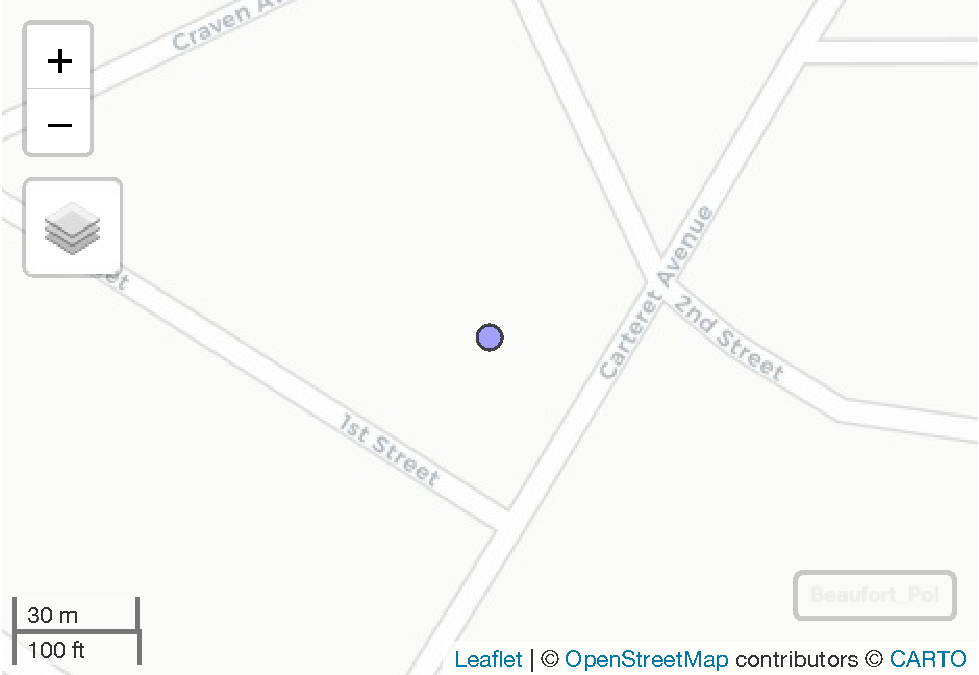
\includegraphics{Project_Template_TLK_files/figure-latex/Map of Beaufort-1.pdf}

\begin{Shaded}
\begin{Highlighting}[]
\CommentTok{\#repeat the steps for the next layer}
\NormalTok{Beaufort\_Town }\OtherTok{\textless{}{-}} \FunctionTok{st\_as\_sf}\NormalTok{(Beaufort\_Pol)}

\FunctionTok{mapview}\NormalTok{(Beaufort\_Town, }\AttributeTok{col.regions =} \StringTok{"red"}\NormalTok{)}
\end{Highlighting}
\end{Shaded}

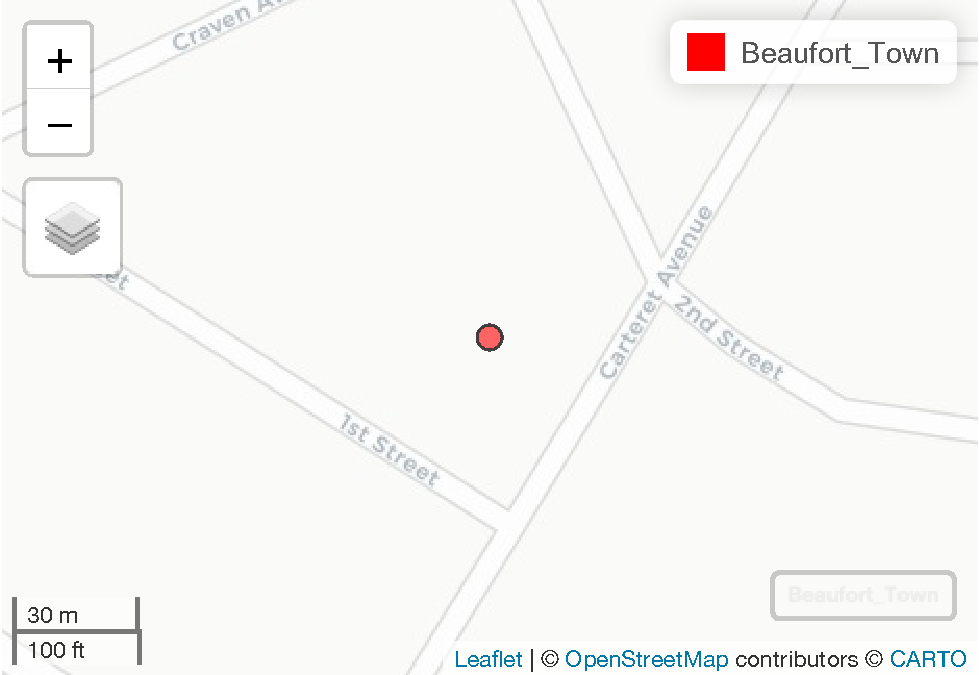
\includegraphics{Project_Template_TLK_files/figure-latex/Map of Beaufort-2.pdf}

\begin{Shaded}
\begin{Highlighting}[]
\CommentTok{\# Load NC counties info }
\NormalTok{NC\_data }\OtherTok{\textless{}{-}} \FunctionTok{st\_read}\NormalTok{(}\StringTok{"./Data/Spatial/cb\_2018\_us\_county\_20m.shp"}\NormalTok{) }\SpecialCharTok{\%\textgreater{}\%} 
  \FunctionTok{filter}\NormalTok{(STATEFP }\SpecialCharTok{==} \DecValTok{37}\NormalTok{)}
\end{Highlighting}
\end{Shaded}

\begin{verbatim}
## Reading layer `cb_2018_us_county_20m' from data source 
##   `/Users/tarokatayama/Desktop/Duke_Semester_2/Environmental_data_analytics/R_Projects/KatayamaNgenziThornton_ENV872_EDA_FinalProject/Data/Spatial/cb_2018_us_county_20m.shp' 
##   using driver `ESRI Shapefile'
## Simple feature collection with 3220 features and 9 fields
## Geometry type: MULTIPOLYGON
## Dimension:     XY
## Bounding box:  xmin: -179.1743 ymin: 17.91377 xmax: 179.7739 ymax: 71.35256
## Geodetic CRS:  NAD83
\end{verbatim}

\begin{Shaded}
\begin{Highlighting}[]
\CommentTok{\# Visualize MC data}
\FunctionTok{mapview}\NormalTok{(NC\_data)}
\end{Highlighting}
\end{Shaded}

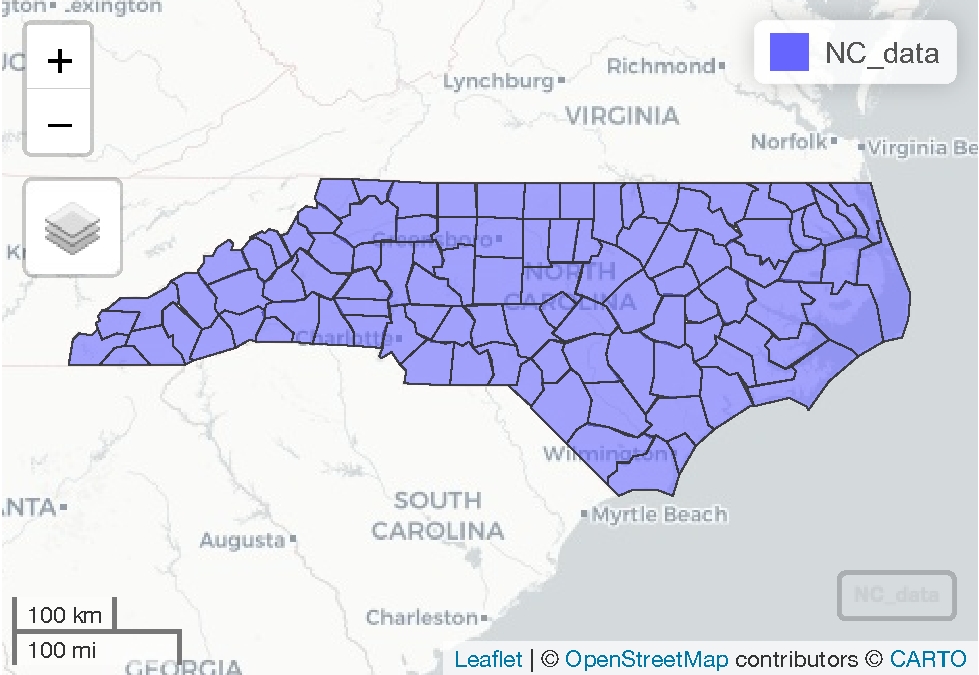
\includegraphics{Project_Template_TLK_files/figure-latex/Map of Beaufort-3.pdf}

\begin{Shaded}
\begin{Highlighting}[]
\CommentTok{\# Filter Beaufort county and map it }
\NormalTok{Beaufort\_County }\OtherTok{\textless{}{-}}\NormalTok{ NC\_data }\SpecialCharTok{\%\textgreater{}\%} 
  \FunctionTok{filter}\NormalTok{(NAME }\SpecialCharTok{\%in\%} \StringTok{"Carteret"}\NormalTok{)}

\FunctionTok{mapview}\NormalTok{(Beaufort\_County, }\AttributeTok{col.regions =} \StringTok{"orange"}\NormalTok{)}
\end{Highlighting}
\end{Shaded}

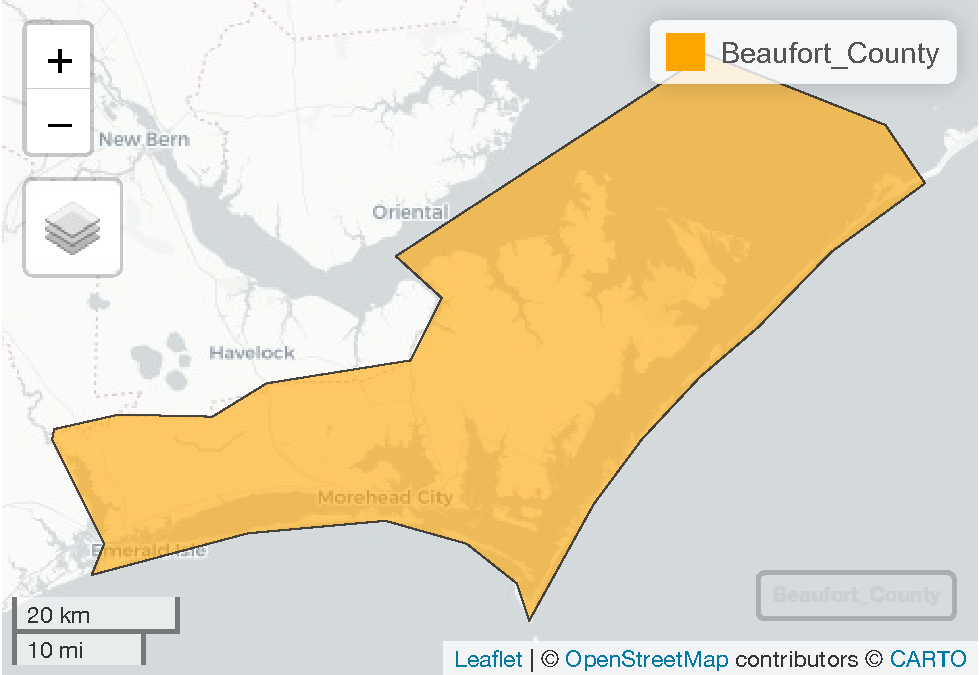
\includegraphics{Project_Template_TLK_files/figure-latex/Map of Beaufort-4.pdf}

\begin{Shaded}
\begin{Highlighting}[]
\CommentTok{\# Combine all map }
\FunctionTok{mapview}\NormalTok{(NC\_data, }\AttributeTok{alpha.regions =} \FloatTok{0.2}\NormalTok{) }\SpecialCharTok{+}
  \FunctionTok{mapview}\NormalTok{(Beaufort\_County, }\AttributeTok{col.regions =} \StringTok{"orange"}\NormalTok{) }\SpecialCharTok{+}
  \FunctionTok{mapview}\NormalTok{(Beaufort\_Town, }\AttributeTok{col.regions =} \StringTok{"red"}\NormalTok{)}
\end{Highlighting}
\end{Shaded}

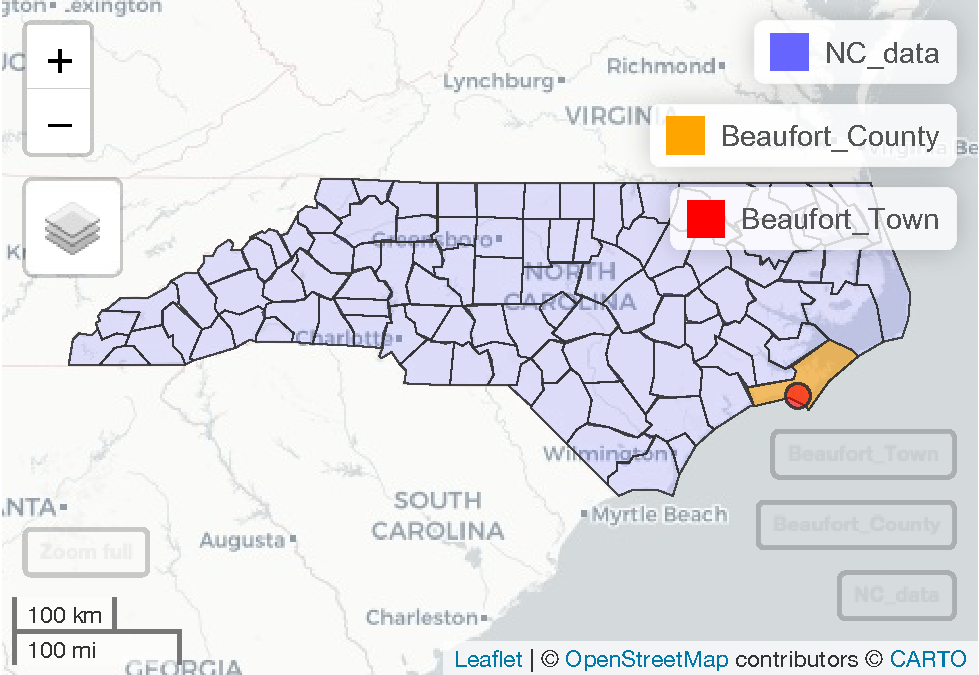
\includegraphics{Project_Template_TLK_files/figure-latex/Map of Beaufort-5.pdf}

\begin{Shaded}
\begin{Highlighting}[]
\CommentTok{\#plot in ggplot to put in presentation }
\FunctionTok{ggplot}\NormalTok{()}\SpecialCharTok{+}
  \FunctionTok{geom\_sf}\NormalTok{(}\AttributeTok{data =}\NormalTok{ NC\_data, }\FunctionTok{aes}\NormalTok{(), }\AttributeTok{alpha=}\FloatTok{0.2}\NormalTok{)}\SpecialCharTok{+}
  \FunctionTok{geom\_sf}\NormalTok{(}\AttributeTok{data =}\NormalTok{ Beaufort\_County, }\AttributeTok{fill=} \StringTok{"orange"}\NormalTok{, }\AttributeTok{alpha =} \FloatTok{0.7}\NormalTok{)}\SpecialCharTok{+}
  \FunctionTok{geom\_sf}\NormalTok{(}\AttributeTok{data=}\NormalTok{ Beaufort\_Town, }\AttributeTok{col =} \StringTok{"red"}\NormalTok{)}
\end{Highlighting}
\end{Shaded}

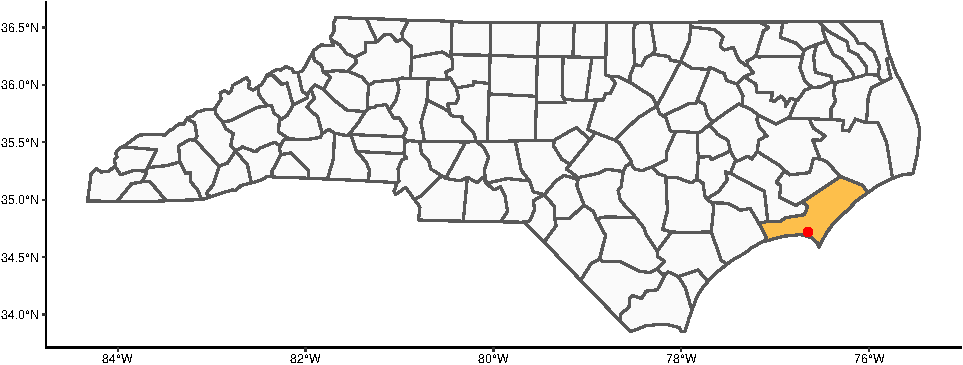
\includegraphics{Project_Template_TLK_files/figure-latex/Map of Beaufort-6.pdf}

\hypertarget{wrangle-data-for-analysis}{%
\section{Wrangle Data for analysis}\label{wrangle-data-for-analysis}}

\begin{Shaded}
\begin{Highlighting}[]
\CommentTok{\#Create a monthly mean precipitation and total monthly precipitation dataset for Beaufort. This dataset is only for visualization purposes. }
\NormalTok{Beaufort\_Clean}\OtherTok{\textless{}{-}}\NormalTok{ Beaufort\_RAW}\SpecialCharTok{\%\textgreater{}\%}
  \FunctionTok{group\_by}\NormalTok{(year,month)}\SpecialCharTok{\%\textgreater{}\%}
   \FunctionTok{summarise}\NormalTok{(}\AttributeTok{meanmonthlyprecip=} \FunctionTok{mean}\NormalTok{(Mean\_Precip\_mm),}
             \AttributeTok{sumMonthlyPrecip=} \FunctionTok{sum}\NormalTok{(Mean\_Precip\_mm))}\SpecialCharTok{\%\textgreater{}\%}
  \FunctionTok{mutate}\NormalTok{(}\AttributeTok{Date=} \FunctionTok{my}\NormalTok{(}\FunctionTok{paste0}\NormalTok{(month,}\StringTok{"{-}"}\NormalTok{, year)))}
\end{Highlighting}
\end{Shaded}

\begin{verbatim}
## `summarise()` has grouped output by 'year'. You can override using the `.groups` argument.
\end{verbatim}

\begin{Shaded}
\begin{Highlighting}[]
\CommentTok{\#Plot precipitation over years to see general trend (Raw dataset). Warning: Plot zoomed in to show trend more clearly; some outliers are not included.}
\FunctionTok{ggplot}\NormalTok{(Beaufort\_RAW, }\FunctionTok{aes}\NormalTok{(}\AttributeTok{x=}\NormalTok{Date, }\AttributeTok{y=}\NormalTok{Mean\_Precip\_mm))}\SpecialCharTok{+}
  \FunctionTok{geom\_line}\NormalTok{()}\SpecialCharTok{+}
  \FunctionTok{ylim}\NormalTok{(}\FunctionTok{c}\NormalTok{(}\DecValTok{0}\NormalTok{,}\DecValTok{80}\NormalTok{))}\SpecialCharTok{+}
  \FunctionTok{labs}\NormalTok{(}\AttributeTok{y=} \StringTok{"Mean Daily Precip (mm)"}\NormalTok{)}\SpecialCharTok{+}
  \FunctionTok{geom\_smooth}\NormalTok{(}\AttributeTok{method=}\NormalTok{lm)}
\end{Highlighting}
\end{Shaded}

\begin{verbatim}
## `geom_smooth()` using formula 'y ~ x'
\end{verbatim}

\begin{verbatim}
## Warning: Removed 53 rows containing non-finite values (stat_smooth).
\end{verbatim}

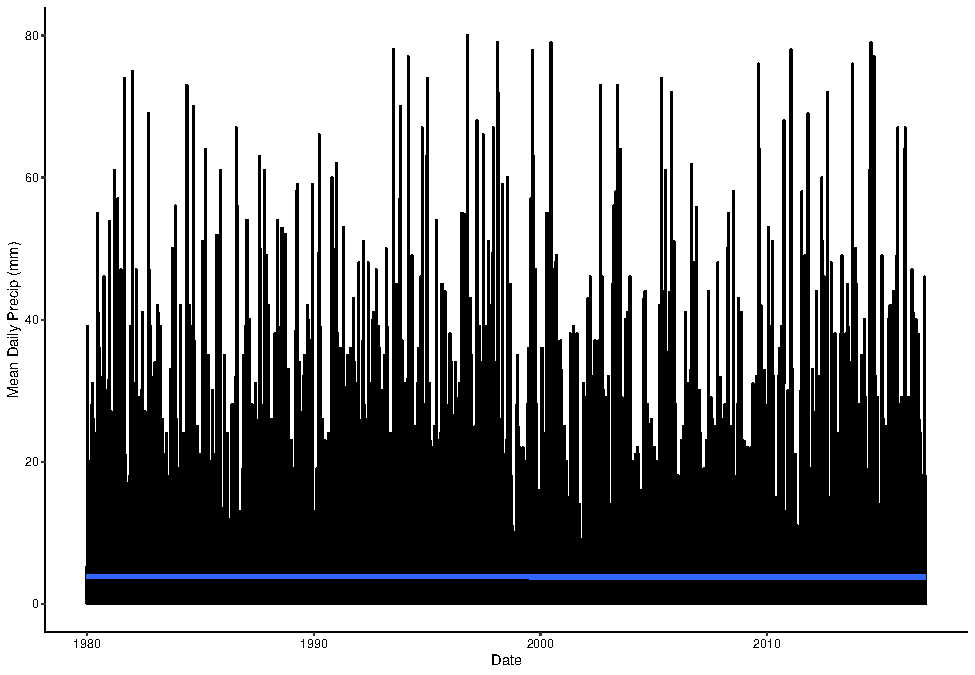
\includegraphics{Project_Template_TLK_files/figure-latex/clean-1.pdf}

\begin{Shaded}
\begin{Highlighting}[]
\CommentTok{\#Plot total monthly precipitation data to see rough trend (Clean dataset)}
\FunctionTok{ggplot}\NormalTok{(Beaufort\_Clean, }\FunctionTok{aes}\NormalTok{(}\AttributeTok{x=}\NormalTok{Date, }\AttributeTok{y=}\NormalTok{sumMonthlyPrecip))}\SpecialCharTok{+}
  \FunctionTok{geom\_line}\NormalTok{()}\SpecialCharTok{+}
  \FunctionTok{labs}\NormalTok{(}\AttributeTok{y=} \StringTok{"Sum Monthly Precip. (mm)"}\NormalTok{)}\SpecialCharTok{+}
  \FunctionTok{geom\_smooth}\NormalTok{(}\AttributeTok{method =}\NormalTok{ lm) }
\end{Highlighting}
\end{Shaded}

\begin{verbatim}
## `geom_smooth()` using formula 'y ~ x'
\end{verbatim}

\begin{verbatim}
## Warning: Removed 9 rows containing non-finite values (stat_smooth).
\end{verbatim}

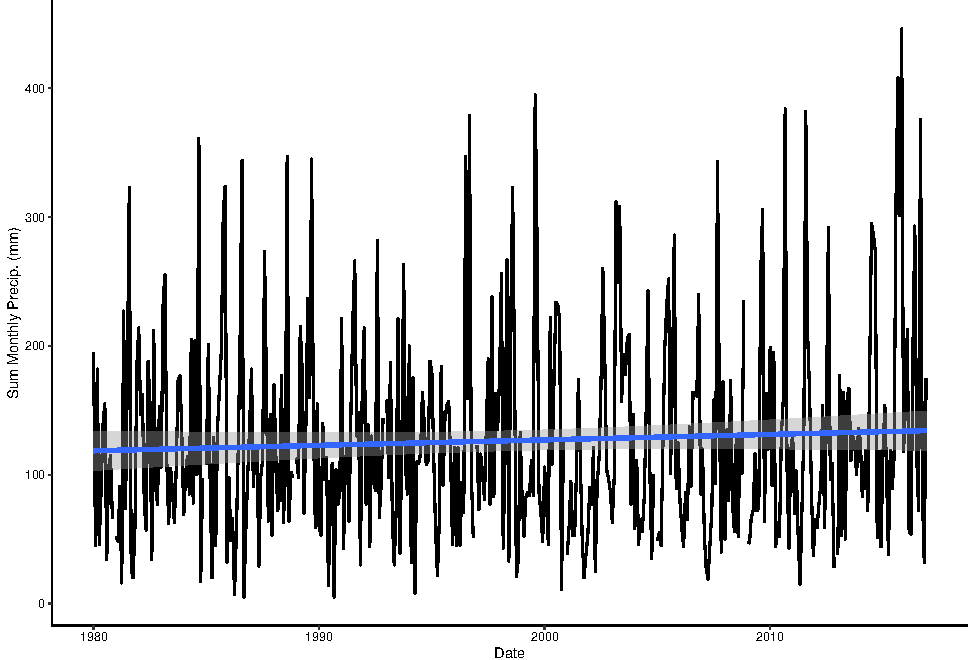
\includegraphics{Project_Template_TLK_files/figure-latex/clean-2.pdf}

\hypertarget{create-a-dataset-for-the-early-decade-1997-2006}{%
\section{Create a dataset for the early decade
(1997-2006)}\label{create-a-dataset-for-the-early-decade-1997-2006}}

\begin{Shaded}
\begin{Highlighting}[]
\CommentTok{\#This dataset has a 10 year time frame with precipitation in inches (1997{-}01{-}01 to 2006{-}12{-}31) and significant 1{-}year/24hr precipitation events in magnitude and number of significant precipitation events}

\NormalTok{Beaufort\_early}\OtherTok{\textless{}{-}}\NormalTok{ Beaufort\_RAW}\SpecialCharTok{\%\textgreater{}\%}
  \FunctionTok{mutate}\NormalTok{(}\AttributeTok{PrecipInches=}\NormalTok{ Mean\_Precip\_mm}\SpecialCharTok{*}\FloatTok{0.0394}\NormalTok{)}\SpecialCharTok{\%\textgreater{}\%}
  \FunctionTok{filter}\NormalTok{(Date }\SpecialCharTok{\textgreater{}}\NormalTok{(}\StringTok{"1996{-}12{-}31"}\NormalTok{), Date }\SpecialCharTok{\textless{}}\NormalTok{ (}\StringTok{"2007{-}01{-}01"}\NormalTok{)) }\SpecialCharTok{\%\textgreater{}\%} 
  \FunctionTok{mutate}\NormalTok{(}\AttributeTok{sigPrecip=} \FunctionTok{ifelse}\NormalTok{(PrecipInches}\SpecialCharTok{\textgreater{}}\FloatTok{3.66}\NormalTok{,PrecipInches,}\DecValTok{0}\NormalTok{),}
         \AttributeTok{NumSigPrecip=} \FunctionTok{ifelse}\NormalTok{(PrecipInches}\SpecialCharTok{\textgreater{}}\FloatTok{3.66}\NormalTok{, }\DecValTok{1}\NormalTok{,}\DecValTok{0}\NormalTok{))}\SpecialCharTok{\%\textgreater{}\%}
  \FunctionTok{select}\NormalTok{(Date , year, month, }
\NormalTok{         day\_of\_month, PrecipInches, sigPrecip, NumSigPrecip)}\SpecialCharTok{\%\textgreater{}\%}
  \FunctionTok{drop\_na}\NormalTok{()}
  
\CommentTok{\#Create a Beaufort early dataset, where non{-}significant 1{-}year/24h precipitation events were classified as NA.}
\NormalTok{Beaufort\_earlyNo0Precip}\OtherTok{\textless{}{-}}\NormalTok{Beaufort\_RAW}\SpecialCharTok{\%\textgreater{}\%}
  \FunctionTok{mutate}\NormalTok{(}\AttributeTok{PrecipInches=}\NormalTok{Mean\_Precip\_mm}\SpecialCharTok{*}\FloatTok{0.0394}\NormalTok{)}\SpecialCharTok{\%\textgreater{}\%}
  \FunctionTok{filter}\NormalTok{(Date }\SpecialCharTok{\textgreater{}}\NormalTok{(}\StringTok{"1996{-}12{-}31"}\NormalTok{), Date }\SpecialCharTok{\textless{}}\NormalTok{ (}\StringTok{"2007{-}01{-}01"}\NormalTok{)) }\SpecialCharTok{\%\textgreater{}\%} 
  \FunctionTok{mutate}\NormalTok{(}\AttributeTok{sigPrecip=} \FunctionTok{ifelse}\NormalTok{(PrecipInches}\SpecialCharTok{\textgreater{}}\FloatTok{3.66}\NormalTok{,PrecipInches,}\ConstantTok{NA}\NormalTok{),}
         \AttributeTok{NumSigPrecip=} \FunctionTok{ifelse}\NormalTok{(PrecipInches}\SpecialCharTok{\textgreater{}}\FloatTok{3.66}\NormalTok{, }\DecValTok{1}\NormalTok{,}\DecValTok{0}\NormalTok{))}\SpecialCharTok{\%\textgreater{}\%}
  \FunctionTok{select}\NormalTok{(Date , year, month, }
\NormalTok{         day\_of\_month, PrecipInches, sigPrecip, NumSigPrecip)}\SpecialCharTok{\%\textgreater{}\%}
  \FunctionTok{drop\_na}\NormalTok{()}

\CommentTok{\#Summary of number of 1{-}year/24hr events per year}
\NormalTok{Beaufort\_early\_summary}\OtherTok{\textless{}{-}}\NormalTok{ Beaufort\_early}\SpecialCharTok{\%\textgreater{}\%}
  \FunctionTok{group\_by}\NormalTok{(year)}\SpecialCharTok{\%\textgreater{}\%}
  \FunctionTok{summarise}\NormalTok{(}\AttributeTok{SigPrecipEvents=} \FunctionTok{sum}\NormalTok{(NumSigPrecip))}

\CommentTok{\#Create a table of number of 1{-}year/24hr events per year.}
\NormalTok{EarlyTable}\OtherTok{\textless{}{-}} \FunctionTok{kable}\NormalTok{(Beaufort\_early\_summary, }\AttributeTok{caption =} \StringTok{"1{-}year/24hr Events Over Year"}\NormalTok{)}
\NormalTok{EarlyTable}
\end{Highlighting}
\end{Shaded}

\begin{longtable}[]{@{}rr@{}}
\caption{1-year/24hr Events Over Year}\tabularnewline
\toprule
year & SigPrecipEvents \\
\midrule
\endfirsthead
\toprule
year & SigPrecipEvents \\
\midrule
\endhead
1997 & 0 \\
1998 & 1 \\
1999 & 1 \\
2000 & 0 \\
2001 & 0 \\
2002 & 0 \\
2003 & 0 \\
2004 & 0 \\
2005 & 1 \\
2006 & 1 \\
\bottomrule
\end{longtable}

\begin{Shaded}
\begin{Highlighting}[]
\CommentTok{\#Create a figure with number and magnitude of significant events per year.}
\NormalTok{Plot\_early\_sig }\OtherTok{\textless{}{-}} \FunctionTok{ggplot}\NormalTok{(Beaufort\_earlyNo0Precip, }\FunctionTok{aes}\NormalTok{(}\AttributeTok{x=}\NormalTok{Date , }\AttributeTok{y=}\NormalTok{sigPrecip))}\SpecialCharTok{+}
  \FunctionTok{geom\_point}\NormalTok{()}\SpecialCharTok{+}
  \FunctionTok{ylim}\NormalTok{(}\FunctionTok{c}\NormalTok{(}\DecValTok{0}\NormalTok{,}\DecValTok{8}\NormalTok{))}\SpecialCharTok{+}
  \FunctionTok{labs}\NormalTok{(}\AttributeTok{y=}\StringTok{"1{-}year/24hr storm events (in)"}\NormalTok{, }\AttributeTok{x=} \StringTok{"Date"}\NormalTok{)}
\NormalTok{Plot\_early\_sig}
\end{Highlighting}
\end{Shaded}

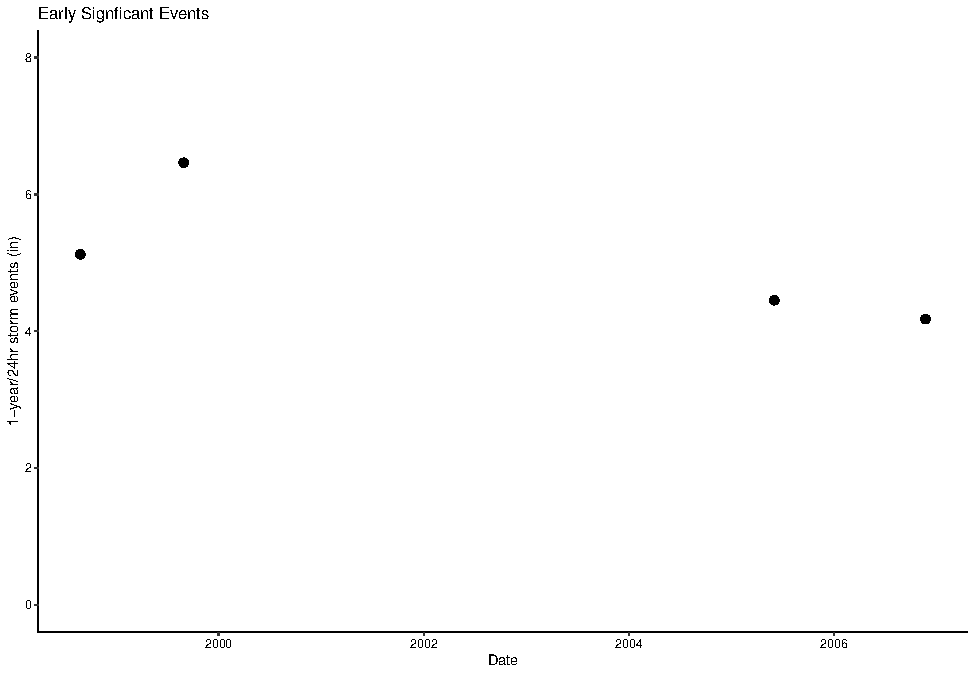
\includegraphics{Project_Template_TLK_files/figure-latex/early-1.pdf}

\begin{Shaded}
\begin{Highlighting}[]
\CommentTok{\#Create a figure showing the overall precipitation for the early decade}
\NormalTok{Plot\_early\_overall }\OtherTok{\textless{}{-}} \FunctionTok{ggplot}\NormalTok{(Beaufort\_early, }\FunctionTok{aes}\NormalTok{(}\AttributeTok{x=}\NormalTok{Date , }\AttributeTok{y=}\NormalTok{PrecipInches))}\SpecialCharTok{+}
  \FunctionTok{geom\_point}\NormalTok{()}\SpecialCharTok{+}
  \FunctionTok{labs}\NormalTok{(}\AttributeTok{y=}\StringTok{"Precipitation (in)"}\NormalTok{, }\AttributeTok{x=} \StringTok{"Date"}\NormalTok{)}
\NormalTok{Plot\_early\_overall}
\end{Highlighting}
\end{Shaded}

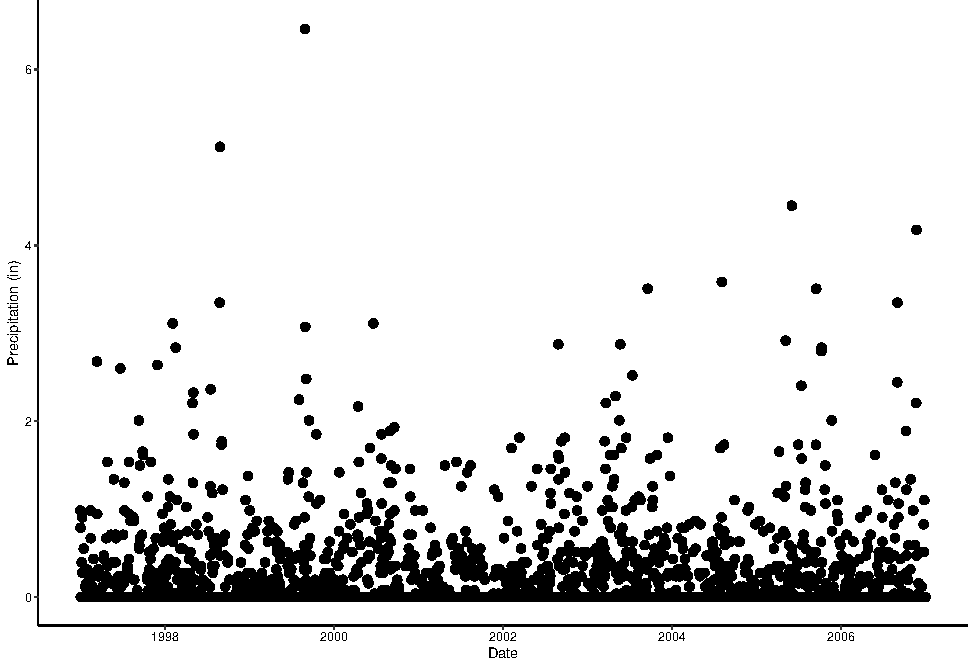
\includegraphics{Project_Template_TLK_files/figure-latex/early-2.pdf}

\hypertarget{create-a-dataset-for-the-late-decade-2007-2016}{%
\section{Create a dataset for the late decade
(2007-2016)}\label{create-a-dataset-for-the-late-decade-2007-2016}}

\begin{Shaded}
\begin{Highlighting}[]
\CommentTok{\#This dataset has a 10 year time frame, precipitation in inches (2007{-}01{-}01 to 2016{-}12{-}30) and significant 1{-}year/24hr precipitation events in magnitude and number of significant precipitation events}

\NormalTok{Beaufort\_Late}\OtherTok{\textless{}{-}}\NormalTok{ Beaufort\_RAW}\SpecialCharTok{\%\textgreater{}\%}
  \FunctionTok{mutate}\NormalTok{(}\AttributeTok{PrecipInches=}\NormalTok{ Mean\_Precip\_mm}\SpecialCharTok{*}\FloatTok{0.0394}\NormalTok{)}\SpecialCharTok{\%\textgreater{}\%}
  \FunctionTok{filter}\NormalTok{(Date }\SpecialCharTok{\textgreater{}} \StringTok{"2006{-}12{-}31"}\NormalTok{)}\SpecialCharTok{\%\textgreater{}\%}
  \FunctionTok{mutate}\NormalTok{(}\AttributeTok{sigPrecip=} \FunctionTok{ifelse}\NormalTok{(PrecipInches}\SpecialCharTok{\textgreater{}}\FloatTok{3.66}\NormalTok{,PrecipInches,}\DecValTok{0}\NormalTok{),}
         \AttributeTok{NumSigPrecip=} \FunctionTok{ifelse}\NormalTok{(PrecipInches}\SpecialCharTok{\textgreater{}}\FloatTok{3.66}\NormalTok{, }\DecValTok{1}\NormalTok{,}\DecValTok{0}\NormalTok{))}\SpecialCharTok{\%\textgreater{}\%}
  \FunctionTok{select}\NormalTok{(Date, year, month, }
\NormalTok{         day\_of\_month, PrecipInches, sigPrecip, NumSigPrecip)}\SpecialCharTok{\%\textgreater{}\%}
  \FunctionTok{drop\_na}\NormalTok{()}

\CommentTok{\#Create a Beaufort late dataset, where non significant 1{-}year/24hr precipitation events were classified as NA.}
\NormalTok{Beaufort\_LateNo0Precip}\OtherTok{\textless{}{-}}\NormalTok{ Beaufort\_RAW}\SpecialCharTok{\%\textgreater{}\%}
  \FunctionTok{mutate}\NormalTok{(}\AttributeTok{PrecipInches=}\NormalTok{ Mean\_Precip\_mm}\SpecialCharTok{*}\FloatTok{0.0394}\NormalTok{)}\SpecialCharTok{\%\textgreater{}\%}
  \FunctionTok{filter}\NormalTok{(Date }\SpecialCharTok{\textgreater{}} \StringTok{"2006{-}12{-}31"}\NormalTok{)}\SpecialCharTok{\%\textgreater{}\%}
  \FunctionTok{mutate}\NormalTok{(}\AttributeTok{sigPrecip=} \FunctionTok{ifelse}\NormalTok{(PrecipInches}\SpecialCharTok{\textgreater{}}\FloatTok{3.66}\NormalTok{,PrecipInches,}\ConstantTok{NA}\NormalTok{),}
         \AttributeTok{NumSigPrecip=} \FunctionTok{ifelse}\NormalTok{(PrecipInches}\SpecialCharTok{\textgreater{}}\FloatTok{3.66}\NormalTok{, }\DecValTok{1}\NormalTok{,}\DecValTok{0}\NormalTok{))}\SpecialCharTok{\%\textgreater{}\%}
  \FunctionTok{select}\NormalTok{(Date, year, month, }
\NormalTok{         day\_of\_month, PrecipInches, sigPrecip, NumSigPrecip)}\SpecialCharTok{\%\textgreater{}\%}
  \FunctionTok{drop\_na}\NormalTok{()}

\CommentTok{\#Summary of number of significant 1{-}year.24hr events per year (Late)}
\NormalTok{Beaufort\_late\_summary}\OtherTok{\textless{}{-}}\NormalTok{ Beaufort\_Late}\SpecialCharTok{\%\textgreater{}\%}
  \FunctionTok{group\_by}\NormalTok{(year)}\SpecialCharTok{\%\textgreater{}\%}
  \FunctionTok{summarise}\NormalTok{(}\AttributeTok{SigPrecipEvents=} \FunctionTok{sum}\NormalTok{(NumSigPrecip))}

\CommentTok{\#Create a figure with number and magnitude of significant 1{-}year/24hr events per year.}
\NormalTok{Plot\_late\_sig }\OtherTok{\textless{}{-}} \FunctionTok{ggplot}\NormalTok{(Beaufort\_LateNo0Precip, }\FunctionTok{aes}\NormalTok{(}\AttributeTok{x=}\NormalTok{Date , }\AttributeTok{y=}\NormalTok{sigPrecip))}\SpecialCharTok{+}
  \FunctionTok{geom\_point}\NormalTok{()}\SpecialCharTok{+}
  \FunctionTok{ylim}\NormalTok{(}\FunctionTok{c}\NormalTok{(}\DecValTok{0}\NormalTok{,}\DecValTok{8}\NormalTok{))}\SpecialCharTok{+}
  \FunctionTok{labs}\NormalTok{(}\AttributeTok{y=}\StringTok{"1{-}year/24h storm events (in) "}\NormalTok{, }\AttributeTok{x=} \StringTok{"Date"}\NormalTok{)}
\NormalTok{Plot\_late\_sig}
\end{Highlighting}
\end{Shaded}

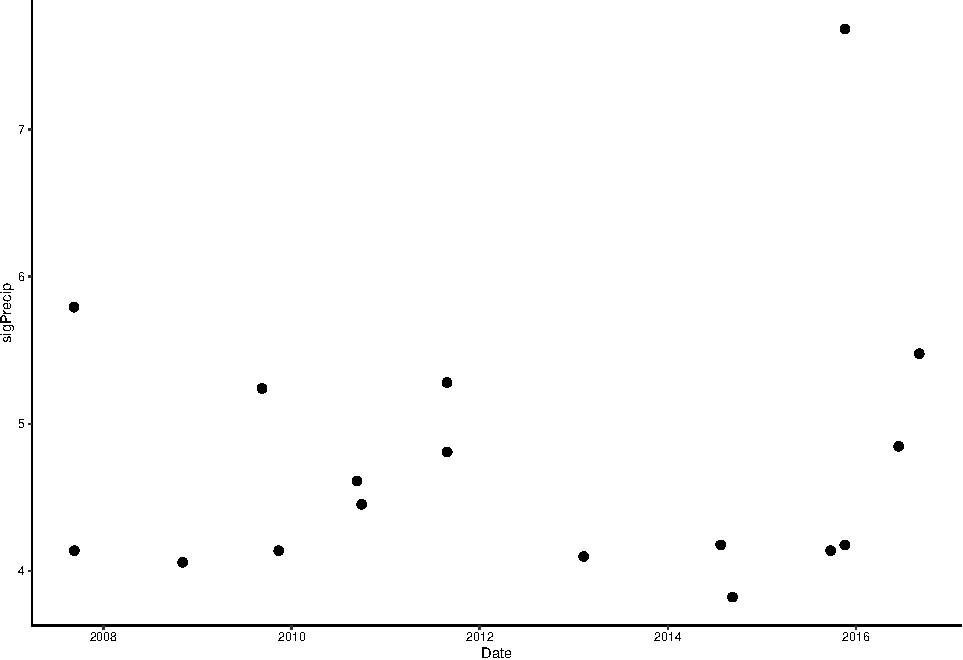
\includegraphics{Project_Template_TLK_files/figure-latex/late-1.pdf}

\begin{Shaded}
\begin{Highlighting}[]
\CommentTok{\#Create a figure showing the overall precipitation for the late decade}
\NormalTok{Plot\_late\_overall }\OtherTok{\textless{}{-}} \FunctionTok{ggplot}\NormalTok{(Beaufort\_Late, }\FunctionTok{aes}\NormalTok{(}\AttributeTok{x=}\NormalTok{Date , }\AttributeTok{y=}\NormalTok{PrecipInches))}\SpecialCharTok{+}
  \FunctionTok{geom\_point}\NormalTok{()}\SpecialCharTok{+}
  \FunctionTok{labs}\NormalTok{(}\AttributeTok{y=}\StringTok{"Precipitation (in)"}\NormalTok{, }\AttributeTok{x=} \StringTok{"Date"}\NormalTok{)}
\NormalTok{Plot\_late\_overall}
\end{Highlighting}
\end{Shaded}

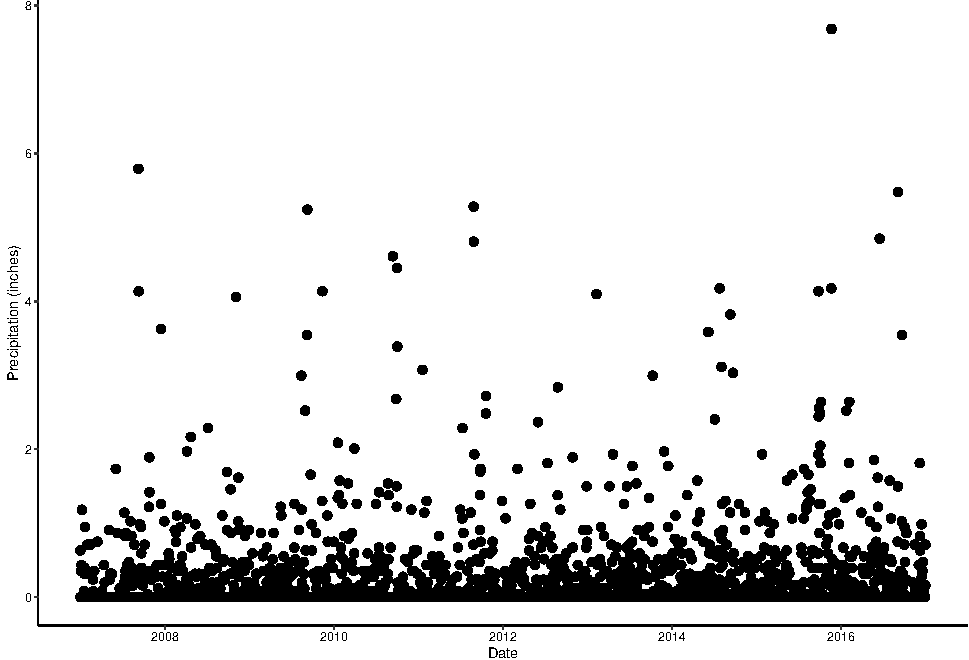
\includegraphics{Project_Template_TLK_files/figure-latex/late-2.pdf}

\begin{Shaded}
\begin{Highlighting}[]
\CommentTok{\#Create a table of number of significant 1{-}year/24hr events per year.}
\NormalTok{LateTable}\OtherTok{\textless{}{-}} \FunctionTok{kable}\NormalTok{(Beaufort\_late\_summary, }\AttributeTok{caption =} \StringTok{"Significant Events Over Year"}\NormalTok{)}
\NormalTok{LateTable}
\end{Highlighting}
\end{Shaded}

\begin{longtable}[]{@{}rr@{}}
\caption{Significant Events Over Year}\tabularnewline
\toprule
year & SigPrecipEvents \\
\midrule
\endfirsthead
\toprule
year & SigPrecipEvents \\
\midrule
\endhead
2007 & 2 \\
2008 & 1 \\
2009 & 2 \\
2010 & 2 \\
2011 & 2 \\
2012 & 0 \\
2013 & 1 \\
2014 & 2 \\
2015 & 3 \\
2016 & 2 \\
\bottomrule
\end{longtable}

\hypertarget{create-a-plot-to-combine-the-1-year24-hour-events-for-each-decade}{%
\section{Create a plot to combine the 1-year/24 hour events for each
decade}\label{create-a-plot-to-combine-the-1-year24-hour-events-for-each-decade}}

\begin{Shaded}
\begin{Highlighting}[]
\FunctionTok{grid.arrange}\NormalTok{(Plot\_early\_sig, Plot\_late\_sig, }\AttributeTok{ncol=}\DecValTok{2}\NormalTok{)}
\end{Highlighting}
\end{Shaded}

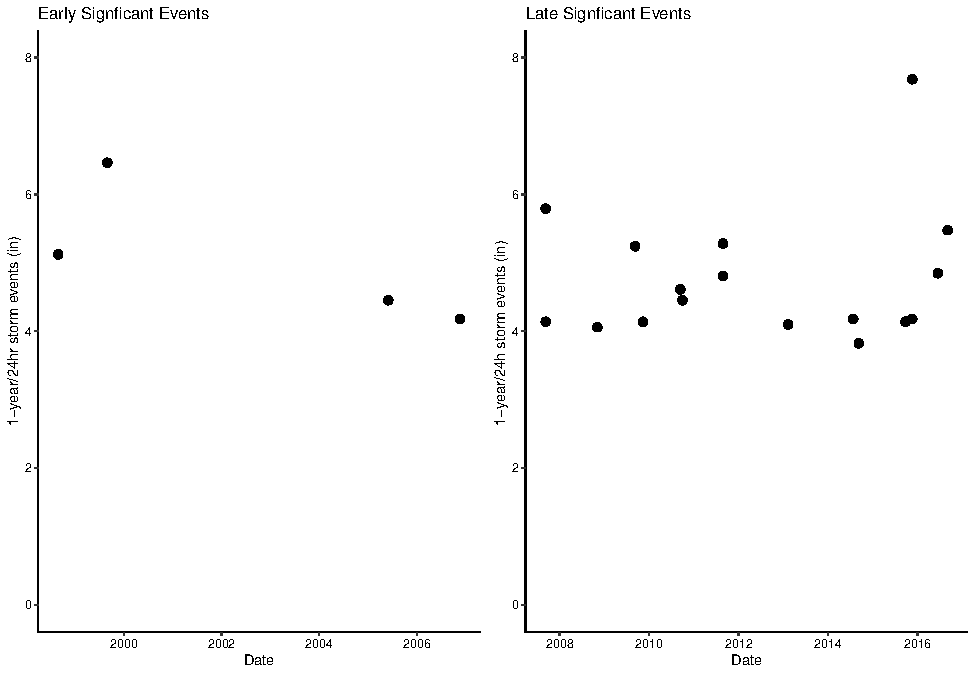
\includegraphics{Project_Template_TLK_files/figure-latex/combined one year storms-1.pdf}

\newpage

\hypertarget{analysis}{%
\section{Analysis}\label{analysis}}

Perform t-test and seasonal Mann-Kendall for overall dataset

\begin{Shaded}
\begin{Highlighting}[]
\FunctionTok{t.test}\NormalTok{(Beaufort\_RAW}\SpecialCharTok{$}\NormalTok{Mean\_Precip\_mm)}
\end{Highlighting}
\end{Shaded}

\begin{verbatim}
## 
##  One Sample t-test
## 
## data:  Beaufort_RAW$Mean_Precip_mm
## t = 43.492, df = 13504, p-value < 2.2e-16
## alternative hypothesis: true mean is not equal to 0
## 95 percent confidence interval:
##  3.953508 4.326684
## sample estimates:
## mean of x 
##  4.140096
\end{verbatim}

\begin{Shaded}
\begin{Highlighting}[]
\CommentTok{\#significant \textless{}{-} This means that there is a significant change in precipitation over the years 1980 to 2016}

\CommentTok{\#Using Seasonal Mann{-}Kendall to look at trend excluding seasonality. This will be a better indicator of significant change than the t{-}test. That being said, both tests were both run.}
\NormalTok{Beaufort\_RAW\_2}\OtherTok{\textless{}{-}}\NormalTok{Beaufort\_RAW}

\CommentTok{\#Used linear interpolation to fill missing data for precipitation data.}
\NormalTok{Beaufort\_RAW\_2}\SpecialCharTok{$}\NormalTok{Mean\_Precip\_mm}\OtherTok{\textless{}{-}}
  \FunctionTok{na.approx}\NormalTok{(Beaufort\_RAW\_2}\SpecialCharTok{$}\NormalTok{Mean\_Precip\_mm)}

\CommentTok{\#Created a time series analysis of the precipitation data at Beaufort.}
\NormalTok{firstday}\OtherTok{\textless{}{-}} \FunctionTok{day}\NormalTok{(}\FunctionTok{first}\NormalTok{(Beaufort\_RAW\_2}\SpecialCharTok{$}\NormalTok{Date))}
\NormalTok{firstmonth}\OtherTok{\textless{}{-}} \FunctionTok{month}\NormalTok{(}\FunctionTok{first}\NormalTok{(Beaufort\_RAW\_2}\SpecialCharTok{$}\NormalTok{Date))}
\NormalTok{firstyear}\OtherTok{\textless{}{-}} \FunctionTok{year}\NormalTok{(}\FunctionTok{first}\NormalTok{(Beaufort\_RAW\_2}\SpecialCharTok{$}\NormalTok{Date))}


\NormalTok{Beaufort\_TS}\OtherTok{\textless{}{-}} \FunctionTok{ts}\NormalTok{(Beaufort\_RAW\_2}\SpecialCharTok{$}\NormalTok{Mean\_Precip\_mm, }
                 \AttributeTok{start =} \FunctionTok{c}\NormalTok{(firstyear, firstmonth, firstday),}
                 \AttributeTok{frequency =} \DecValTok{365}\NormalTok{)}

\CommentTok{\#Decomposed the time series to see components.}
\NormalTok{Beaufort\_decompose}\OtherTok{\textless{}{-}} \FunctionTok{stl}\NormalTok{(Beaufort\_TS, }\AttributeTok{s.window =} \StringTok{"periodic"}\NormalTok{)}
\FunctionTok{plot}\NormalTok{(Beaufort\_decompose)}
\end{Highlighting}
\end{Shaded}

\includegraphics{Project_Template_TLK_files/figure-latex/t-test Overall\& Seasonal Mann-Kendall Ovearall-1.pdf}

\begin{Shaded}
\begin{Highlighting}[]
\CommentTok{\#Ran a seasonal Mann Kendall to see if there is a change in precipitation over the time of the data frame. Used seasonal Mann{-}Kendall to exclude seasonality of precipitation. }
\NormalTok{Beaufort.trend}\OtherTok{\textless{}{-}}\NormalTok{Kendall}\SpecialCharTok{::}\FunctionTok{SeasonalMannKendall}\NormalTok{(Beaufort\_TS)}
\NormalTok{Beaufort.trend}
\end{Highlighting}
\end{Shaded}

\begin{verbatim}
## tau = 0.0189, 2-sided pvalue =0.0056612
\end{verbatim}

\begin{Shaded}
\begin{Highlighting}[]
\CommentTok{\#Significant! \textless{}{-} This means that when you exclude seasonality there is still a significant change in precipitation from 1980 to 2016}
\end{Highlighting}
\end{Shaded}

T-test was run to compare the two decades

\begin{Shaded}
\begin{Highlighting}[]
\CommentTok{\#Here we are looking to see if there is a change in precipitation amount comparing two decades (1999{-}2006) \& (2007{-}2016)}
\FunctionTok{t.test}\NormalTok{(Beaufort\_early}\SpecialCharTok{$}\NormalTok{PrecipInches, Beaufort\_Late}\SpecialCharTok{$}\NormalTok{PrecipInches)}
\end{Highlighting}
\end{Shaded}

\begin{verbatim}
## 
##  Welch Two Sample t-test
## 
## data:  Beaufort_early$PrecipInches and Beaufort_Late$PrecipInches
## t = -0.64906, df = 7133.8, p-value = 0.5163
## alternative hypothesis: true difference in means is not equal to 0
## 95 percent confidence interval:
##  -0.02812072  0.01413102
## sample estimates:
## mean of x mean of y 
## 0.1627598 0.1697546
\end{verbatim}

\begin{Shaded}
\begin{Highlighting}[]
\CommentTok{\#not significant\textless{}{-} meaning precipitation amount not significantly different over the two decades}

\CommentTok{\#Here we compared the significant 1{-}year/24hr precipitation events for the two decades (1999{-}2006) \& (2007{-}2016).}
\FunctionTok{t.test}\NormalTok{(Beaufort\_early}\SpecialCharTok{$}\NormalTok{sigPrecip, Beaufort\_Late}\SpecialCharTok{$}\NormalTok{sigPrecip)}
\end{Highlighting}
\end{Shaded}

\begin{verbatim}
## 
##  Welch Two Sample t-test
## 
## data:  Beaufort_early$sigPrecip and Beaufort_Late$sigPrecip
## t = -2.7068, df = 5451.7, p-value = 0.006815
## alternative hypothesis: true difference in means is not equal to 0
## 95 percent confidence interval:
##  -0.028681849 -0.004586864
## sample estimates:
##   mean of x   mean of y 
## 0.005537589 0.022171945
\end{verbatim}

\begin{Shaded}
\begin{Highlighting}[]
\CommentTok{\#significant!\textless{}{-} There are more statistically significant 1 year precipitation events in later decade. }
\end{Highlighting}
\end{Shaded}

\begin{Shaded}
\begin{Highlighting}[]
\CommentTok{\# There is not autocorrelation, although the first 3 show a statistically significant autocorrelation trend of precipitation.}
\FunctionTok{acf}\NormalTok{(Beaufort\_TS) }
\end{Highlighting}
\end{Shaded}

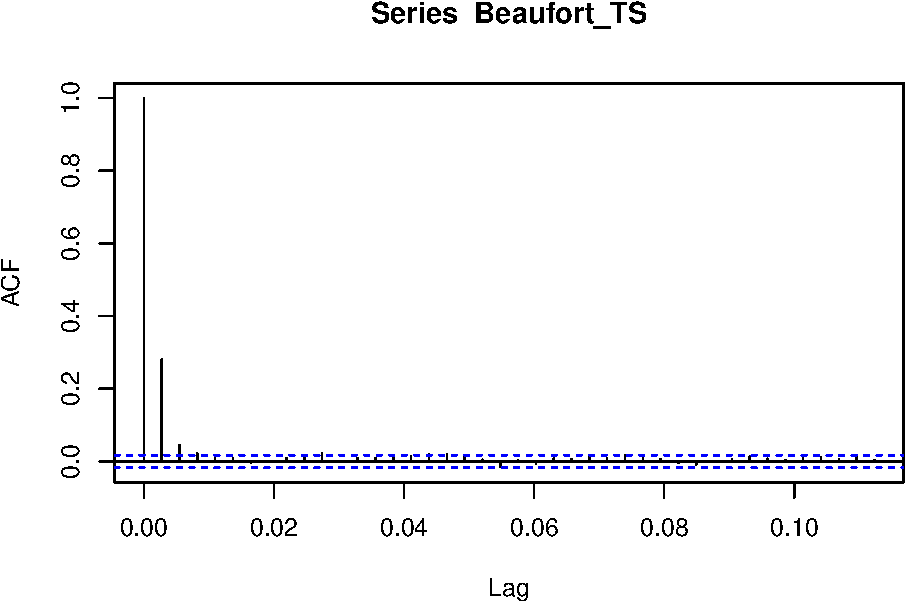
\includegraphics{Project_Template_TLK_files/figure-latex/unnamed-chunk-2-1.pdf}

\begin{Shaded}
\begin{Highlighting}[]
\FunctionTok{pacf}\NormalTok{(Beaufort\_TS) }
\end{Highlighting}
\end{Shaded}

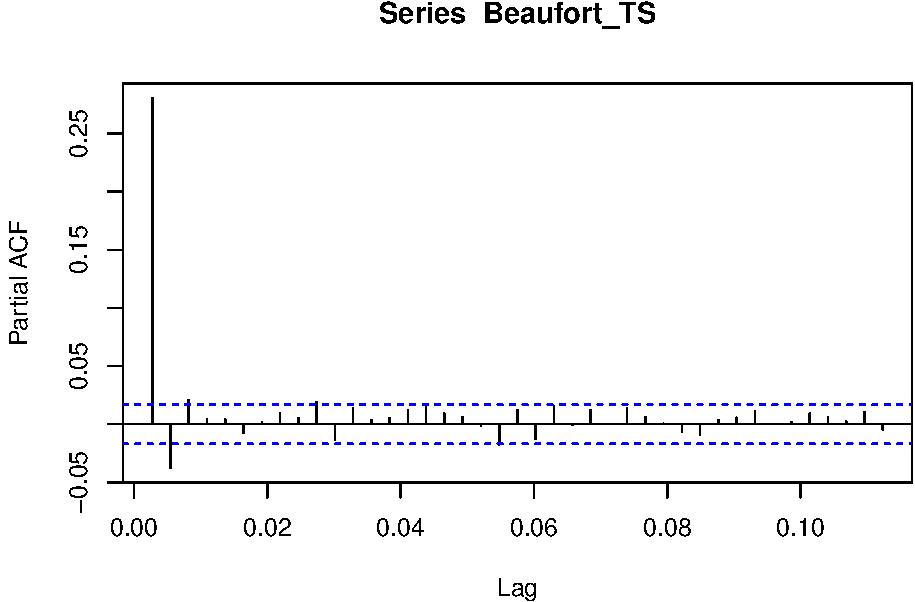
\includegraphics{Project_Template_TLK_files/figure-latex/unnamed-chunk-2-2.pdf}

\begin{Shaded}
\begin{Highlighting}[]
\CommentTok{\#No autocovariance, despite the first 3 lag time are statistically significant while others are not. And the second one is negative partial autocorrelation. }
\end{Highlighting}
\end{Shaded}

\newpage

\hypertarget{summary-and-conclusions}{%
\section{Summary and Conclusions}\label{summary-and-conclusions}}

After careful analysis, it has been concluded that there is a
significant increase in precipitation from 1980 to 2016 in Beaufort, NC.
When comparing decade 1 (1997 to 2006) to decade 2 (2007 to 2016) there
was no significant increase in precipitation.That being said, when
looking at significant 1-year/24hr storm events with a threshold of 3.66
inches there was a significant increase from decade 1 to decade 2.

While there isn't enough information to draw conclusions based on
precipitation alone, our prediction is climate change as the driver
behind the increase in 1-year/24hr storm events between decades.

Large storm events are important to track in future climate change
studies.

\end{document}
